% last updated in April 2002 by Antje Endemann
% Based on CVPR 07 and LNCS, with modifications by DAF, AZ and elle, 2008 and AA, 2010, and CC, 2011; TT, 2014; AAS, 2016

\documentclass[runningheads]{llncs}
\usepackage{graphicx}
\usepackage{amsmath,amssymb} % define this before the line numbering.
\usepackage{algorithm}
\usepackage{algpseudocode}
\usepackage{ruler}
\usepackage{color}
\usepackage[width=122mm,left=12mm,paperwidth=146mm,height=193mm,top=12mm,paperheight=217mm]{geometry}
\begin{document}
% \renewcommand\thelinenumber{\color[rgb]{0.2,0.5,0.8}\normalfont\sffamily\scriptsize\arabic{linenumber}\color[rgb]{0,0,0}}
% \renewcommand\makeLineNumber {\hss\thelinenumber\ \hspace{6mm} \rlap{\hskip\textwidth\ \hspace{6.5mm}\thelinenumber}}
% \linenumbers
\pagestyle{headings}
\mainmatter
\def\ECCV16SubNumber{***}  % Insert your submission number here

\title{Unsupervised Deep Domain Adaptation on People Detection} % Replace with your title

\titlerunning{ECCV-16 submission ID \ECCV16SubNumber}

\authorrunning{ECCV-16 submission ID \ECCV16SubNumber}

\author{Anonymous ECCV submission}
\institute{Paper ID \ECCV16SubNumber}


\maketitle

\begin{abstract}
This paper addresses the problem of unsupervised domain adaptation on the task of people detection in crowded scenes. That is, given a deep detection model well-trained on source domain, we adapt it into scene-specific detectors for any target domain on which no annotations are available. Firstly, we utilize iterative algorithm to iteratively auto-annotate target samples with high confidence on people instance as training set for scene-specific model on target domain. However, auto-annotated samples not only are lack of negative samples, but contains false positive samples. Therefore, on the one hand, we reuse negative samples from source domain to compensate for imbalance between the amount of positive samples and negative samples. On the other hand, we design an unsupervised regularizer based on deep network to mitigate influence from data error. Besides, we transform the last full connected layer into two sub-layers-- element-wise multiply layer and sum layer, on which the unsupervised regularizer can be added on. In experiments on people detection, the proposed method boosts recall by nearly $30\%$ while precision stays almost the same. Furthermore, we perform our method on standard domain adaptation benchmarks on both supervised and unsupervised settings and our results are state of the art.

\keywords{Unsupervised Domain Adaptation, Unsupervised Regularizer, Deep Neural Network, People Detection}
\end{abstract}


\section{Introduction}

Deep neural network has shown great power on traditional computer vision tasks, however, the labelled dataset should be large enough to train a deep model. In famous challenges such as PASCAL VOC and MS COCO, millions of labelled images are needed for training. This is also the case in surveillance applications. The annotation process for the task of people detection in crowded scenes is even more resource consuming, cause we need to label concrete locations of people instances. In modern society, there are over millions of cameras deployed for surveillance. However, these surveillance situations vary in lights, background, viewpoints, camera resolutions and so on. Directly utilizing models trained on old scenes will results in poor performance on the new situations due to data distribution changes. It is also unpractice to annotate people instances for every surveillance situation.

When there are few or even none of labelled data in target domain, domain adaptation helps to reduce the amount of labelled data needed. Most traditional works \cite{saenko2010adapting,kulis2011you,gopalan2011domain,huang2006correcting,gretton2009covariate} either learn a shared representation between source and target domain, or project features into a common subspace. Recently, there are also works \cite{wang2014scene,zeng2014deep,hattori2015learning} proposed to learn a scene-specific detector by deep architectures. However, these approaches are heuristic either on constructing feature space or re-weighting samples. Our motivation of developing a domain adaptation architecture is to reduce heuristic methods required during adaptation process.

In this paper, we proposed a new approach of unsupervised deep domain adaptation on people detection. Using source model trained on source domain as initialization, we utilize iterative algorithm to iteratively auto-annotate target examples with high confidence as people instance on target domain for the first iteration. During each iteration, these auto-annotated data are regarded as training set to update target model, which, then, can be taken as the auto-annotation tool to auto-annotate target samples for the next iteration. However, these auto-annotated samples are defective, including lack of negative samples and existence of false positive samples, which will no doubt lead to exploration of predictions on non-people instances. Therefore, on the one hand, to compensate for the quantitative imbalance between positive and negative samples, we randomly sample negative instances from source domain and mix into training set. On the other hand, based on deep network, we design an unsupervised regularizer to mitigate influence from data error and avoid overfitting. To have better regularization effect during adaptation process, we transform the last full connected layer of deep model into two sub-layers, element-wise multiply layer and sum layer. Thus, the unsupervised regularizer can be added on element-wise multiply layer to adjust all weights in the deep network and gain better performance.

Also, we further evaluate our approach on standard domain adaptation benchmark Office Dataset. The results of our adaptation approach outperform previously published works on both supervised and unsupervised scenarios, which also demonstrate the feasibility of our adaptation approach on both detection and classification tasks.

The contributions of our work are three folds.
\begin{itemize}
\item We proposed a feasible scheme to learn scene-specific deep detectors for target domains by unsupervised methodology, which can be easily deployed to various surveillance situations without any additional annotations.
\item For better performance of unsupervised regularizer, we transform the last full connected layer of deep network into two sub-layers, element-wise layer and sum layer. Thus, all weights contained in the deep network can be adjusted under the unsupervised regularizer. To our knowledge, this is the first attempt to transform full connected layers for the purpose of domain adaptation.
\item Experiments on standard domain adaptation benchmarks for classification also demonstrate the applicability of our approach to other deep domain adaptation tasks.
\end{itemize}

The remainder of this paper is organized as follows. Section \ref{section:Relate Work} reviews related works. Section \ref{section:Our Approach} presents the details of our approach. Experimental results are shown in Section \ref{section:Experiment Results}. Section \ref{section:Conclusions} concludes the paper.

\section{Relate Work}
\label{section:Relate Work}

In many detection works, generic model trained by large amount of samples on source domain are directly utilized to detect on target domain. They assume that samples on target domain are subsets of source domain. However, when the distribution of data on target and source domain varies largely, the performance will drop significantly. Domain adaptation aims to reduce the amount of data needed for target domain.

Many domain adaptation works tried to learn a common representation space shared between source and target domain. Saenko et al. \cite{saenko2010adapting,kulis2011you} proposed a both linear-transform-based technique and kernel-transform-based technique to minimize domain changes. Gopalan et al. \cite{gopalan2011domain} projected features into Grassmann manifold instead of operating on features of raw data. Alternatively, Mesnil et al. \cite{mesnil2012unsupervised} used transfer learning to obtain good representations. However, these methods are limited because scene-specific features are not learned to boost accuracy. The regularizer of our method are inspired these works.

Another group of works \cite{huang2006correcting,gretton2009covariate,gong2013connecting} on domain adaptation is to make the distribution of source and target domain more similar. Among these works, Maximum Mean Discrepancy (MMD) is used to as a metric to reselect samples from source domain in order to have similar distribution as target samples. In \cite{ghifary2014domain}, MMD is incorporated as regularization to reduce distribution mismatch.

There are also works on deep adaptation to construct scene-specific detector. Wang et al.\cite{wang2014scene} explored context cues to compute confidence, and \cite{zeng2014deep} learns distributions of target samples and proposed a cluster layer for scene-specific visual patterns. These works re-weighted auto-annotated samples for their final object function and additional context cues are needed for reliable performance. However, heuristic methods are required to re-weight samples. Alternately, Hattori el al. \cite{hattori2015learning} learned scene-specific detector by generating a spatially-varying pedestrian appearance model. And Pishchulin et al. \cite{pishchulin2011learning} used 3D shape models to generate training data. However, Synthesis for domain adaptation are also costly. Our approach minimize heuristic algorithms needed during adaptation process.


\section{Our Approach}
\label{section:Our Approach}

In this section, we introduce our unsupervised domain adaptation architecture on the task of people detection in crowded scenes. Under the unsupervised setting, we use iterative algorithm to iteratively auto-annotate target samples and update target model. As the auto-annotated samples contain data error, the performance decline caused by false positive samples will exceed the performance boost resulting from true positive samples if the target model is trained only with detection loss function. Therefore, an unsupervised regularizer is required to mitigate the influence from data error on target model. Based on the assumption that source domain and target domain should share the same feature space after feature extraction layers, we encode an unsupervised regularizer to make a constraint that the distribution of data representation on the element-wise multiply layer should be similar between source stream and target stream.

The adaptation architecture of our approach consists of two streams -- source stream and target stream, as shown in Fig \ref{fig:streams}. Source steam takes samples from source domain as input, while target stream are trained by auto-annotated positive samples from target domain and negative samples from source domain. These two streams can utilize any deep detection network as their basic model, as well as their detection loss function as supervised loss functions of two streams. In our experiment, we use the detection network mentioned in Section \ref{section:Detection Network} as the basic model. For the purpose of unsupervised regularizer, the last full connected layers on both source and target model are transformed into two sub-layers -- element-wise multiply layer and sum layer, as mentioned in Section \ref{section:Element-wise Multiply Layer}.

\begin{figure}
\centering
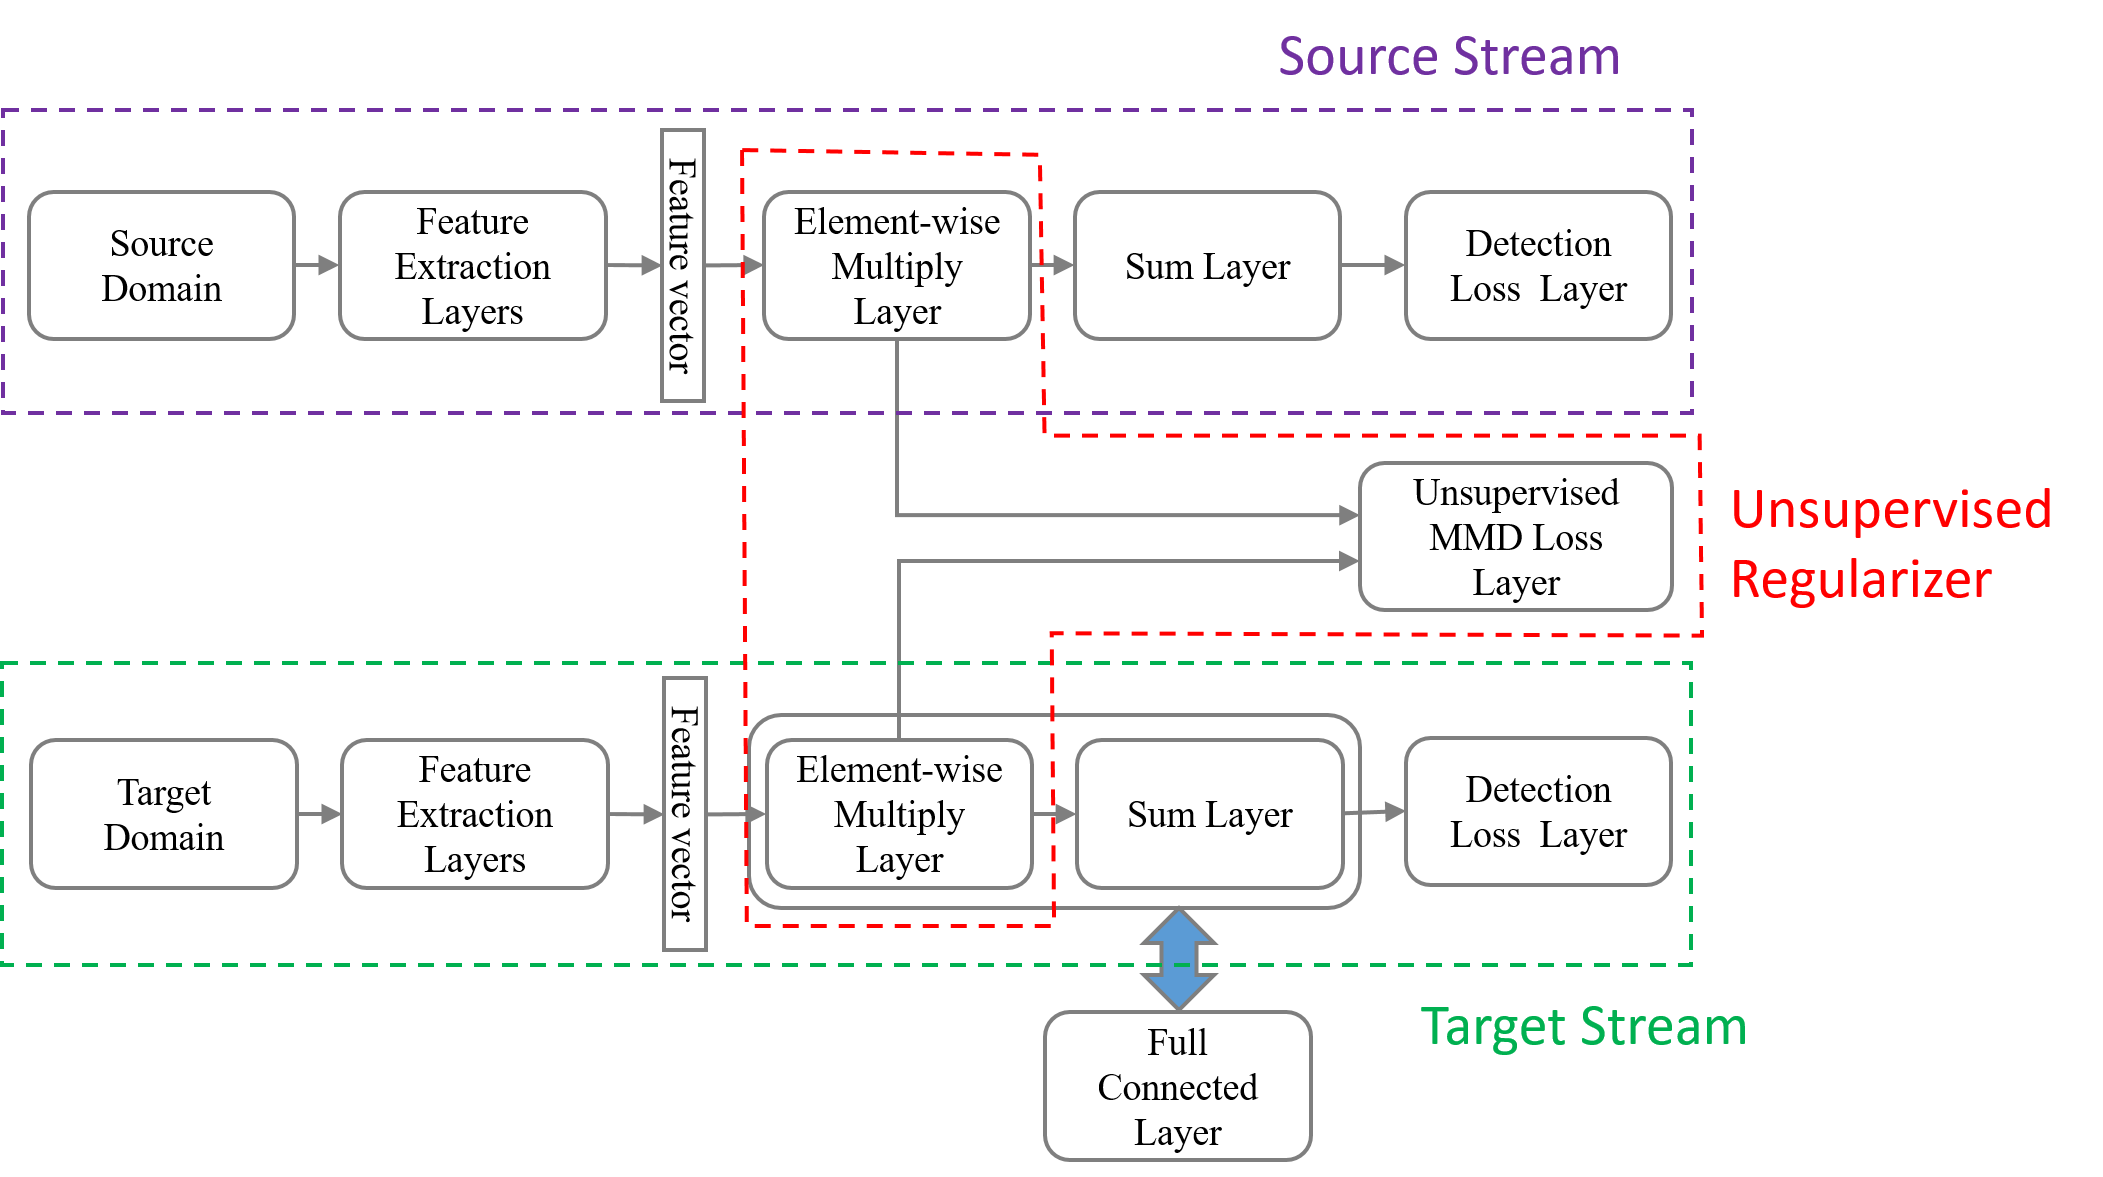
\includegraphics[height=6.5cm]{images/streams.png}
\caption{xxxxxxxxxxxxxxxxxxxxxxxxx}
\label{fig:streams}
\end{figure}

The loss function of adaptation architecture is composed of a supervised loss and an unsupervised regularizer. We denote training samples from source domain as ${\bf X}^{S} = \{x^{S}_{i}\}^{N^{S}}_{i=1}$. For training samples on source domain, we have corresponding annotations $Y^{S} = \{y^{S}_{i}\}^{N^{S}}_{i=1}$ with $y^{S}_{i} = (b^{S}_{i},l^{S}_{i})$, where $b^{S}_{i} = (x,y,w,h) \in R^{4}$ is the bounding box location and $l^{S}_{i} \in \{0,1\}$ is the label indicating whether $x^{S}_{i}$ is a people instance. At $n^{th}$ adaptation iteration, we have two set of training samples, auto-annotated positive samples from target domain ${\bf X}^{T,n} = \{x^{T,n}_{j}\}^{N^{T,n}}_{j=1}$ and tantamount negative samples from source domain ${\bf X}^{S,n} = \{x^{S,n}_{k}\}^{N^{T,n}}_{k=1}$. Their corresponding annotations can be denoted as $Y^{T,n} = \{y^{T,n}_{j}\}^{N^{T,n}}_{j=1}$ and $Y^{S,n} = \{y^{S,n}_{k}\}^{N^{T,n}}_{k=1}$ with $y^{T,n}_{j} = (b^{T,n}_{j},l^{T,n}_{j}\equiv1,c^{T,n}_{j})$, and $y^{S,n}_{k} = (b^{S,n}_{k},l^{S,n}_{k}\equiv0)$, respectively. $c^{T,n}_{*}$ is the confidence given by auto-annotation tools and $N^{I}$ is the maximum number of adaptation iterations. Now we can formulate the combination of supervised loss and unsupervised regularizer as follows:
\begin{eqnarray}
% \nonumber to remove numbering (before each equation)
  L(\theta^{T,n}|{\bf X}^{T,n},{\bf Y}^{T,n},{\bf X}^{S,n},{\bf Y}^{S,n},{\bf X}^{S},\theta^{S}) = L_{S} + \alpha * L_{U} \\
 \nonumber  L_{S} = \sum^{N^{T,n}}_{j=1}{\sigma(c^{T,n}_{j})* ( R(\theta^{T,n}|x^{T,n}_{j},b^{T,n}_{j})+C(\theta^{T,n}|x^{T,n}_{j},l^{T,n}_{j}) )} \\
             + \sum^{N^{T,n}}_{k=1}{( R(\theta^{T,n}|x^{S,n}_{k},b^{S,n}_{k})+C(\theta^{T,n}|x^{S,n}_{k},l^{S,n}_{k}) )}\\
  L_{U} = L_{EWM}(\theta^{T}|{\bf X}^{T},{\bf X}^{S},\theta^{S}) \label{Eq:lmmd}
\end{eqnarray}
where $L_{S}$ is supervised loss to learn the scene-specific detector and $L_{U}$ is the unsupervised regularizer part. $\sigma(\cdot)$ is a step function to re-weight supervised loss of auto-annotated data. $R(\cdot)$ is a regression loss for bounding box location, such as norm-1 loss, and $C(\cdot)$ is a classification loss for bounding box confidence, such as cross-entropy loss. And $L_{EWM}(\cdot)$, to be introduced in Section \ref{section:Element-wise Multiply Layer}, is the MMD-based loss added on the element-wise multiply layer for unsupervised regularization. $\alpha$ is the coefficient balancing the effect of supervised and unsupervised loss.


\subsection{Iterative Algorithm}
\label{Section:Iterative Algorithm}

Iterative algorithm is the training method of the target stream of our adaptation architecture. There are two reasons to employ iterative algorithm. Firstly, auto-annotated data on target domain vary for every adaptation iteration and new positive samples will be auto-annotated as training set. Compared to methods without iterative algorithm, it helps to avoid overfitting caused by lack of data. Besides, unsupervised regularizer performs better with more training data as it's a distribution based regularizer.

There are two stages for iterative algorithm. Source stream and target stream are separately trained at different stages. At initialization stage, source model of source stream are trained under supervised loss function with abundant labelled data, ${\bf X}^{S}$, from source domain. After its convergence, the weights of source model $\theta^{S}$ are taken to initialize target stream. At adaptation stage, target model is trained by auto-annotated data under both supervised loss function and unsupervised regularizer. Note that we do not jointly train two streams at adaptation stage and the weights of source model stays static which is served as a distribution reference for unsupervised regularizer at adaptation stage. The complete adaptation process is illustrated in Algorithm \ref{algorithm:Deep domain adaptation algorithm (to be completed)}. After a predetermined iteration limit $N^{I}$ is reached, we obtain our final detection model on the target domain.

\begin{algorithm}
\caption{Deep domain adaptation algorithm (to be completed)}
\label{algorithm:Deep domain adaptation algorithm (to be completed)}
\begin{algorithmic}[1]
\Procedure{Deep domain adaptation} {} \\
\indent Train source model on source stream with abundant annotated data \\
\indent Use well-trained source model on source stream to initialize target model on target stream as $M_{0}$
\For{i = 0:$N^{I}$} \\
\indent \indent $M_{i}$ generate auto-annotated positive samples ${\bf X}^{T,n}$ of target domain with ${\bf Y}^{T,n}$\\
\indent \indent Randomly sampled negative instances ${\bf X}^{S,n}$ from source domain with ${\bf Y}^{S,n}$\\
\indent \indent ${\bf X}^{n} = \{{\bf X}^{T,n}, {\bf X}^{S,n}\}$ \\
\indent \indent ${\bf Y}^{n} = \{{\bf Y}^{T,n}, {\bf Y}^{S,n}\}$ \\
\indent \indent Take (${\bf X}^{n}$, ${\bf Y}^{n}$) as training data to upgrade $M_{i}$ into $M_{i+1}$
\EndFor \\
\indent $M_{N^{I}}$: final model.
\EndProcedure
\end{algorithmic}
\end{algorithm}

Different from source domain, we use auto-annotation tools to auto-annotate people instances with high confidence as training set on target domain. At first iteration, we take source model as the auto-annotation tool. For subsequent adaptation iterations, updated target model from last adaptation iteration are utilized as the auto-annotation tool. During every adaptation iteration, the auto-annotation tool (also the target model) will be updated. Thus, the training samples for target domain at $n^{th}$ adaptation iteration may differ from that at $(n+1)^{th}$ adaptation iteration.

Note that these auto-annotated data are all regarded as positive samples. That is, we encourage the network to have more confidence on positive instances and stay conservative toward negative instances. This policy will no doubt resulting predictions of many non-people instance and impeding the further training when many non-people instances are regarded as people instances by the target model. To compensate for lack of negative instances, equal amount of negative samples are randomly selected from target domain, which are human annotated and can thus provide true negative samples. To further mitigate influence from data error in auto-annotated data, we will introduce an unsupervised regularizer in Section \ref{Section:Unsupervised weights regularizer on Element-wise Multiply Layer}.


\subsection{Unsupervised weights regularizer on Element-wise Multiply Layer}
\label{Section:Unsupervised weights regularizer on Element-wise Multiply Layer}

\subsubsection{Element-wise Multiply Layer}
\label{section:Element-wise Multiply Layer}
In deep neural network, the last feature vector layer are taken as an important data representation of input images. However, in this paper, we take one step further to focus on the last full connected layer which serves as an decoder to decode rich information of the last feature vector into final outputs. As source model are trained with abundant labelled data on source domain, the parameters of the last full connected layer are also well converged. A regularizer on the last full connected layer can adjust all weights of the network compared with that on the last feature vector layer. Denote the last feature vector, weights of the last full connected layer and final outputs as ${\bf F}_{(1\times N^{D})}$, ${\bf C}_{(N^{D}\times N^{O})}$ and ${\bf P}_{(1\times N^{O})}$, respectively. $ N^{D}, N^{O}$ are the dimension of feature vector and the dimension of output layer, respectively. The operation of the full connected layer can be thus formulated as matrix multiply:
\begin{eqnarray}
% \nonumber to remove numbering (before each equation)
  {\bf P} &=& {\bf F}*{\bf C} \\
  P_{o} &=&  \sum_{d}{F_{d}*C_{d,o}}
\end{eqnarray}
Inspired by this form, we separate the above formula into two sub-operations -- element-wise multiply and sum, which can be formulated as:
\begin{eqnarray}
% \nonumber to remove numbering (before each equation)
  \vec{m}_{o} &=& [F_{d} * C_{d,o}]^{N^{D}}_{d=1} \\
  P_{o} &=& \sum{\vec{m}_{o}}
\end{eqnarray}
where ${\bf M}_{(N^{O}\times N^{D})} = [\vec{m}_{o}]$ is the intermediate results of element-wise multiply operations. $\vec{m}_{o}$ is a vector with $N^{D}$ dimensions, which will be the object of unsupervised regularizer. Finally, we can equivalent-transform the last full connected layer between the last feature vector layer and final outputs layer into element-wise multiply layer and sum layer. The transformed element-wise multiply layer is thus the last layer with weights before output layers. Fig \ref{fig:elementwiselayer} illustrates the transform.

\begin{figure}
\centering
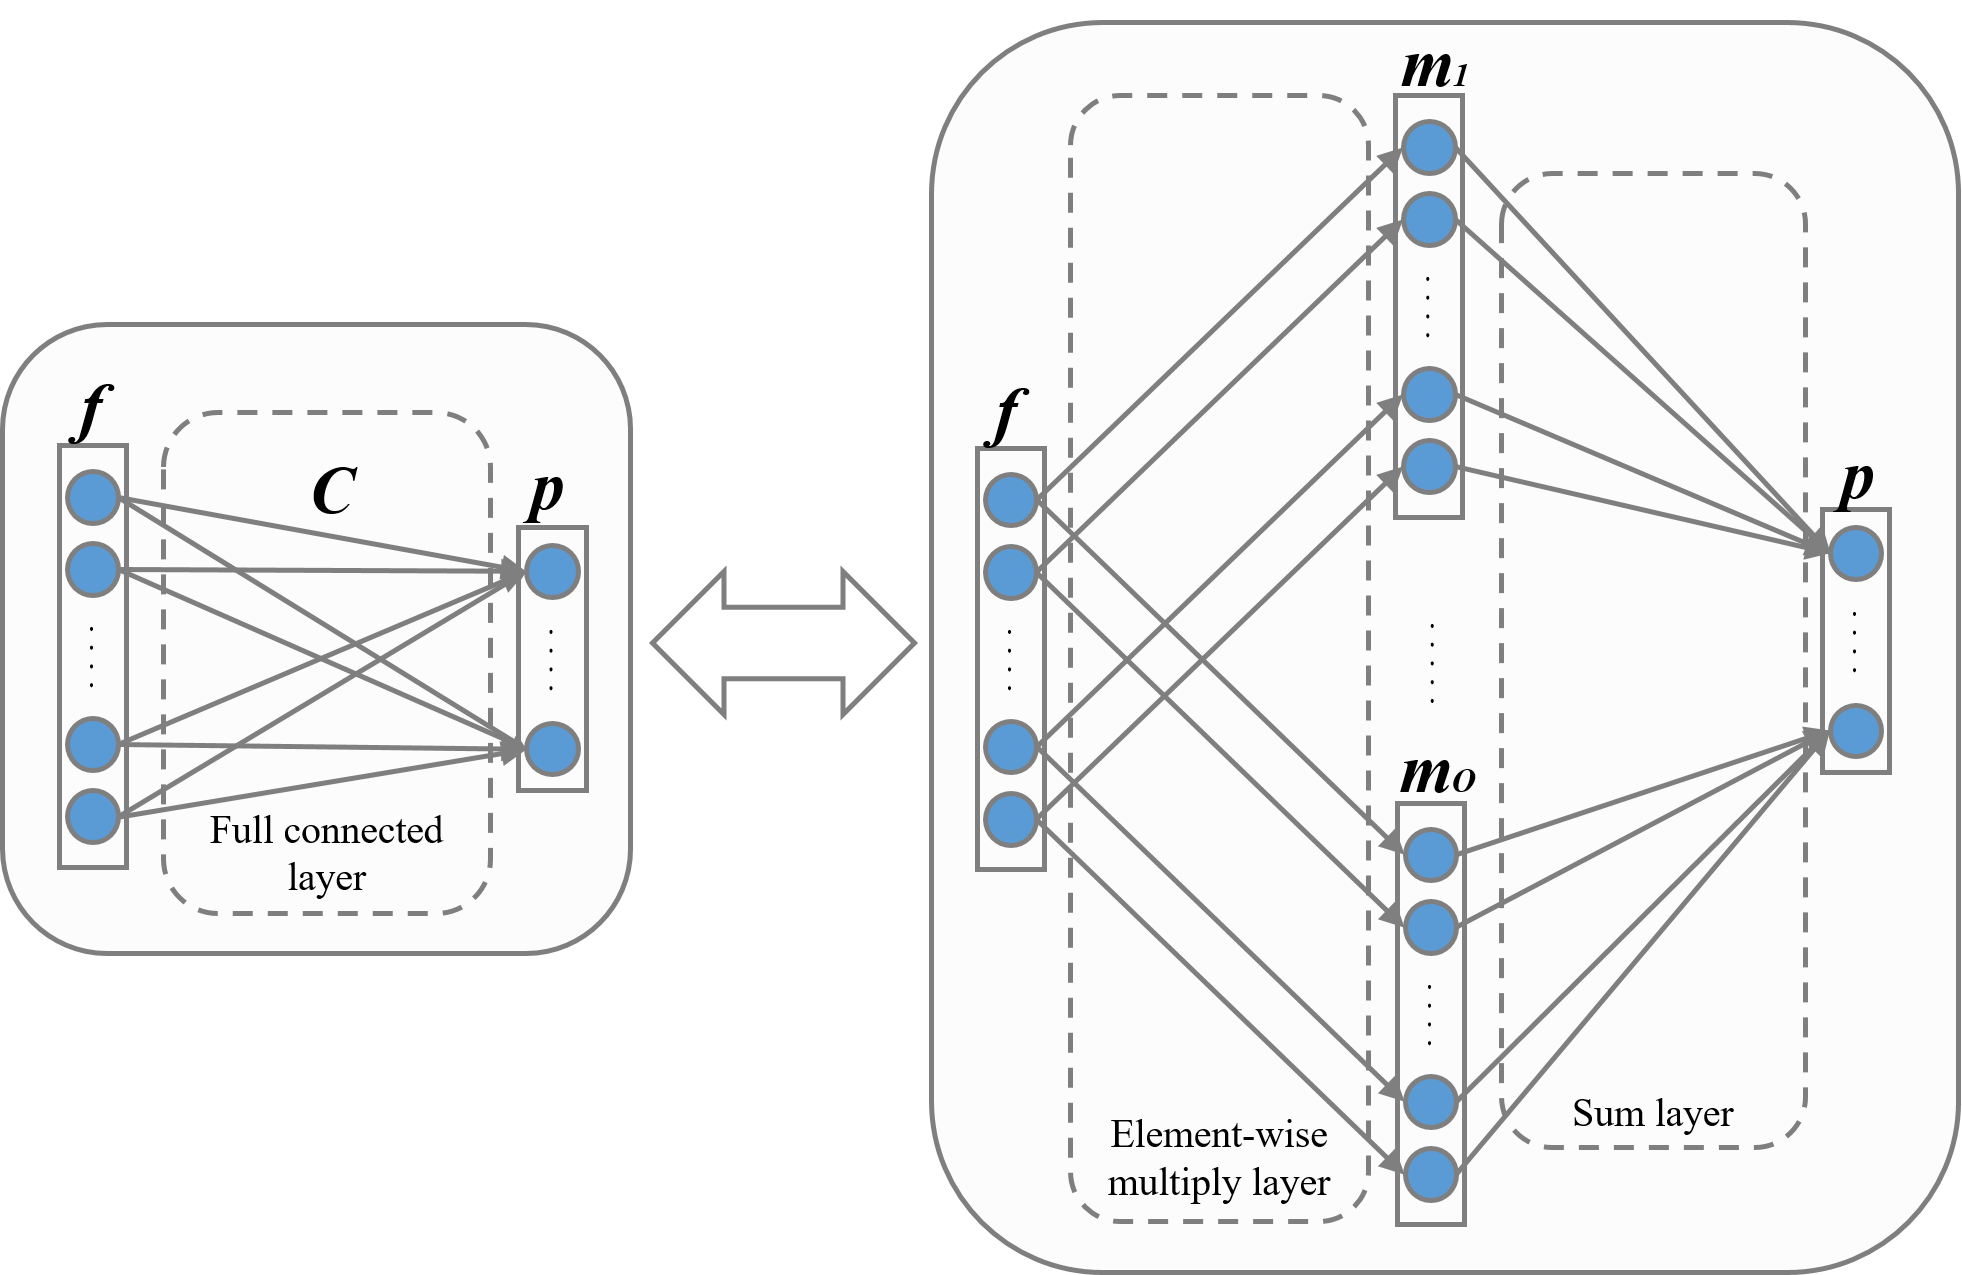
\includegraphics[height=6cm]{images/elementwiselayer.png}
\caption{xxxxxxxxxxxxxx}
\label{fig:elementwiselayer}
\end{figure}

\subsubsection{Unsupervised regularizer on Element-wise Multiply Layer}

This section introduces our unsupervised regularizer. As stated in Section \ref{Section:Iterative Algorithm}, there are false positive samples among auto-annotated data, which will mislead the network and result in worse performance. Thus, we designed an unsupervised regularizer to mitigate the influence. We have the assumption that the dimensions of element-wise multiply layer of the last full connected layer has well converged under the training of abundant source samples. Thus, when the tasks are similar, the distribution of data representations of element-wise multiply layer on source domain and target domain should also be similar. When we train with false positive samples, they are easier to mutate the distribution of data representations. This idea can be illustrated in Fig x(!), balabala.... Confining that the distribution of data representations between source and target domain to be similar helps to reduce the influence caused by data error to some extent. To encode this similarity, we utilize MMD (maximum mean discrepancy) to compute distance between distributions of element-wise multiply layer of source domain and target domain:
\begin{equation}\label{equation:LMMD}
  L_{EWM}(\theta^{T,n}|{\bf X}^{S},{\bf X}^{T,n},\theta^{S}) = \frac{1}{N^{O}} \sum^{N^{O}}_{o=1}{ \parallel \frac{\sum^{N^{T,n}}_{j=1}{(\vec{m}^{T,n}_{o}|x^{T,n}_{j})}}{N^{T,n}} - \frac{\sum^{N^{S}}_{i=1}{(\vec{m}^{S}_{o}|x^{S}_{i})}}{N^{S}} {\parallel}^{2}  }
\end{equation}
which can also interpreted as the Euclidean distance between the center of $\vec{m}^{T,n}_{o}$ and $\vec{m}^{S}_{o}$ across all output dimensions. It's unpractical to get the distribution of the whole training set, while too few images cannot obtain a stable distribution for regularization. In our experiments, the $L_{EWM}(\cdot)$ loss is calculated for every batch. An example comparison of centers of $\vec{m}^{S}_{o}$ of different batches are shown in Fig x(1).

\begin{figure}
\centering
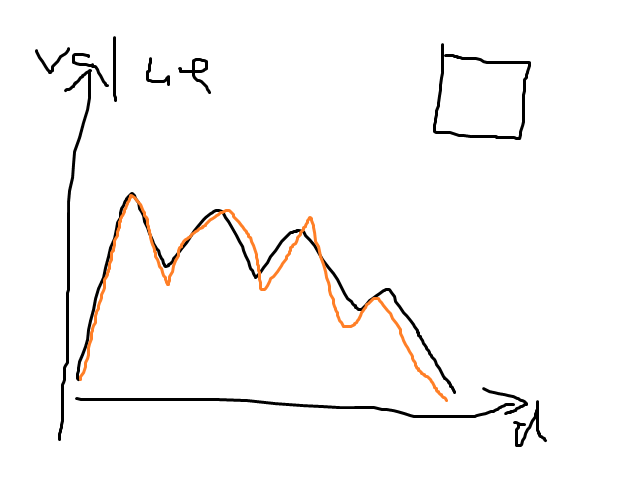
\includegraphics[height=4.5cm]{images/mmd.png}
\caption{One kernel at $x_s$ ({\it dotted kernel}) or two kernels at
$x_i$ and $x_j$ ({\it left and right}) lead to the same summed estimate
at $x_s$. }
\label{fig:example}
\end{figure}


\subsection{Detection Network}
\label{section:Detection Network}
The generic model \footnote{Proposed by Russel et al.} used in our adaptation architecture for source and target stream is an end to end detection network without any precomputed region proposals needed. It consists of a GoogLeNet \cite{szegedy2015going} for feature extraction and a RNN-based decoder for output of bounding box and corresponding confidence, as shown in Fig x(!). Firstly, the GoogLeNet model encode the image into a feature map (15x20x1024) of which each 1024 dimension vector are data representation of its receptive field corresponding to a subregion of the image. Then the RNN-based layers with batch size 300 will decode the data representation and sequentially predict 5 possible bounding boxes by the order of its corresponding confidence. Finally, all outputs are summarized to give final detection results. When trained with abundant samples from source domain, the obtained model has a high precision on target domain, however, its recall is low. Also, different from other detection network \cite{girshick2015fast,vu2015context}, which need precomputed proposals for classification and fine regression, this generic model directly predict bounding boxes with high confidence. Thus, negative instances may contain people and non-people predictions, and cannot be employed in adaptation training.

\begin{figure}
\centering
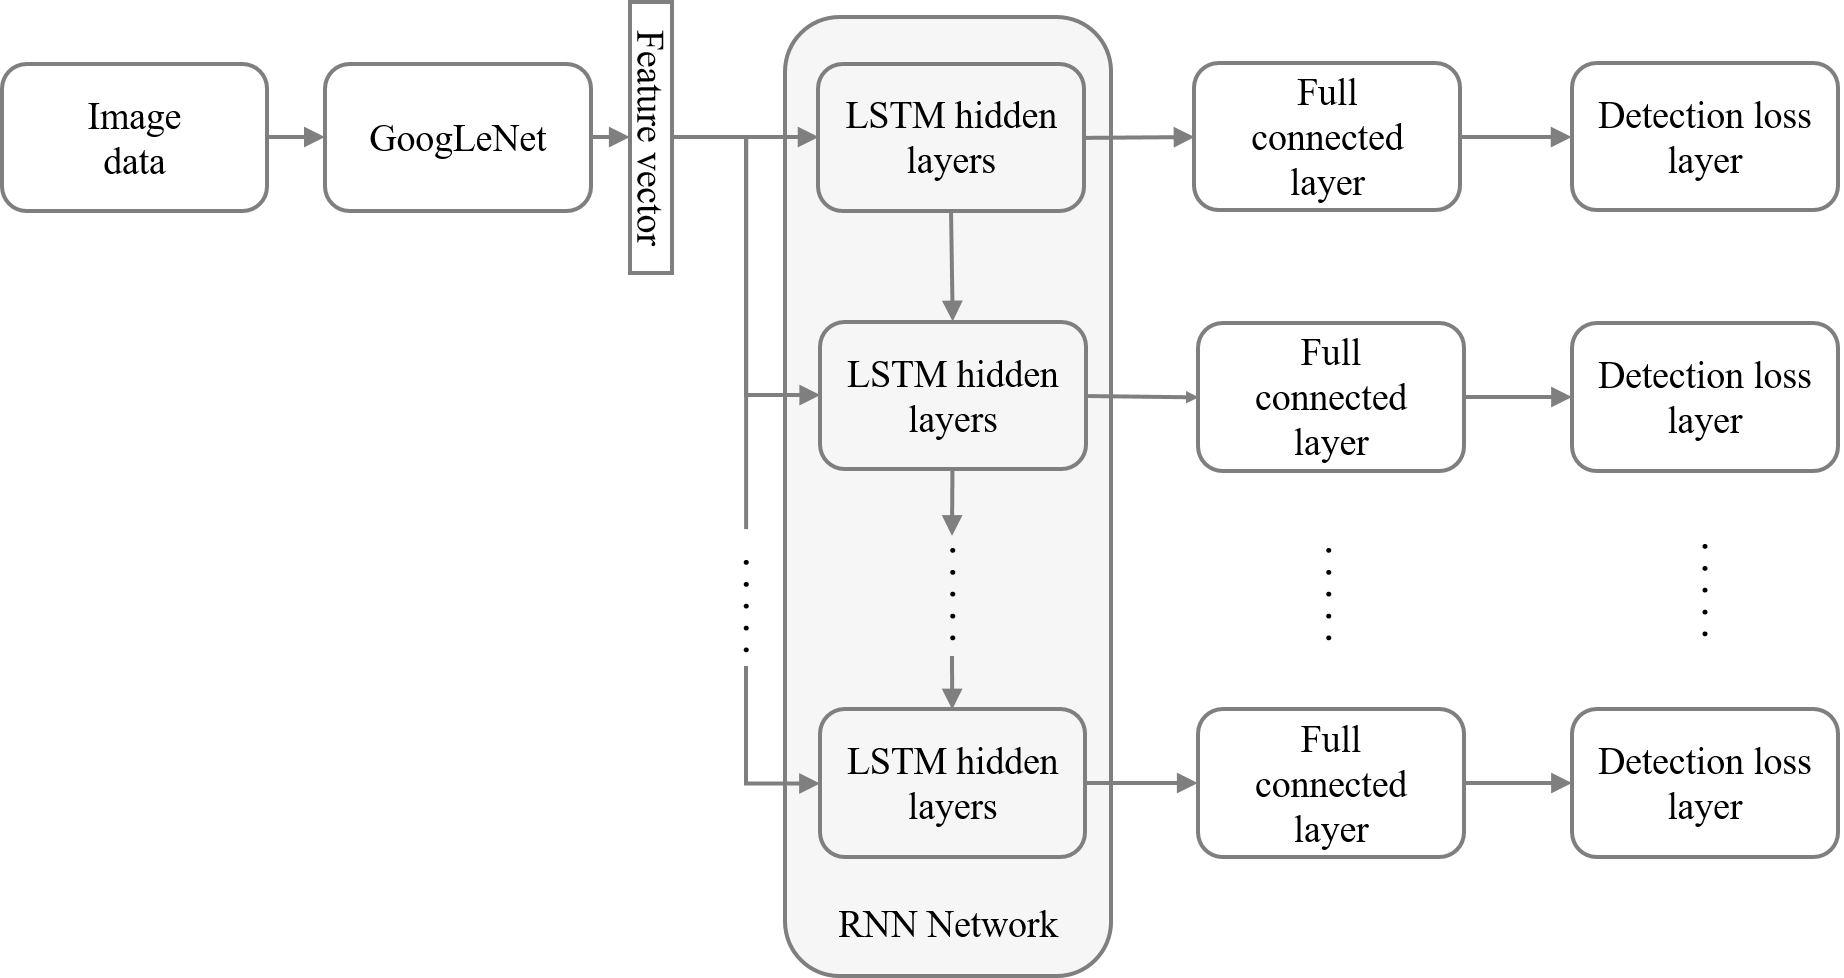
\includegraphics[height=5cm]{images/reinspect.png}
\caption{xxxxxxxxxxxxx}
\label{fig:reinspect}
\end{figure}


\section{Experiment Results}
\label{section:Experiment Results}

In this section, we introduce experiment results on both surveillance applications and standard domain adaptation dataset. Our motivation for unsupervised domain adaptation method is for easier deployment of  We firstly evaluate our approach on video surveillance. Then we employ our approach to standard domain adaptation benchmarks on both supervised and unsupervised settings to demonstrate the effectiveness of our method.

\begin{figure}
\centering
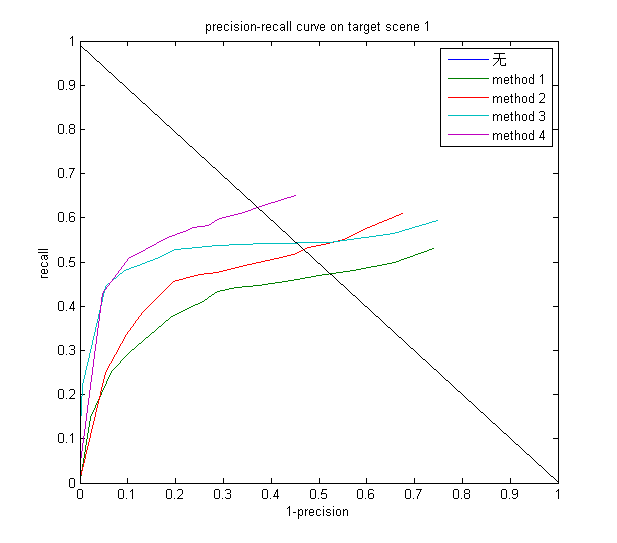
\includegraphics[height=9.5cm]{images/precisionrecallcurve.png}
\caption{xxxx}
\label{fig:precisionrecallcurve}
\end{figure}

\begin{figure}
\centering
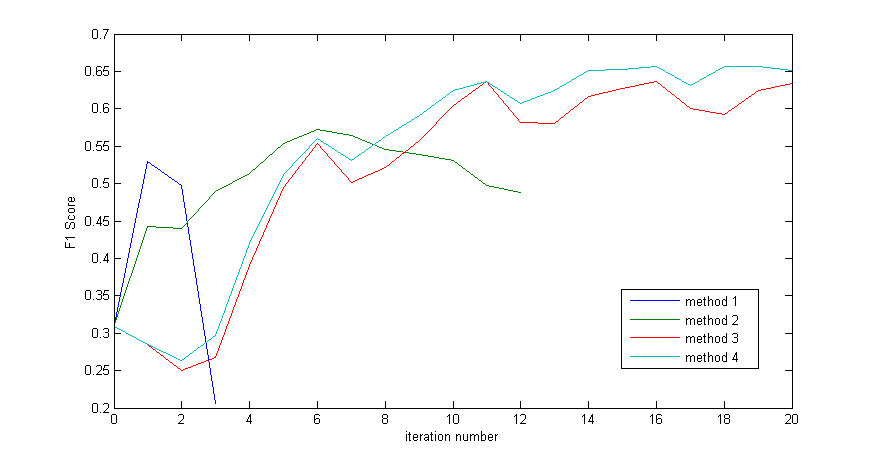
\includegraphics[height=6.5cm]{images/f1score.png}
\caption{xxxx}
\label{fig:precisionrecallcurve}
\end{figure}

\subsection{Domain Adaptation on Crowd Dataset}

\subsubsection{Dataset and evaluation metrics}
To show the effectiveness of our domain adaptation approach on people detection, we collected a dataset consisting of 3 target scenes for target domain. These three scenes contain 1308, 1213 and 331 un-annotated images with 0000, 0000, 0000 people instances respectively. For each scene, 100 images are annotated for evaluation. Instead of labelling the whole body of a person, we labels the head of a person as bounding box during training. The motivation for labelling only people heads comes from detection of indoor people or in crowded scenes, where the body of a person may be invisible. The dataset for source domain are Brainwash Dataset released on http://d2.mpi-inf.mpg.de/datasets. Brainwash Dataset consists of over 11917 images from 3 crowded scenes. Examples of images from source and target domain are shown in Fig x(!).

Our evaluation metrics for detection uses the protocol defined in PASCAL VOC \cite{everingham2015pascal}. To judge a predicted bounding box whether correctly matches a ground truth bounding box, their intersection over their union must exceed 50\%. And Multiple detections of the same ground truth bounding box are regarded as one correct prediction. We plot the precision-recall curve in Fig x(!). Also, the F1 score $F1 = 2*precision*recall/(precision+recall)$ during the adaptation process are also shown in Fig x(!).



\subsubsection{Experimental settings}
We use deep learning framework Caffe \cite{jia2014caffe} as the adaptation architecture of our approach. During the adaptation, we set learning rate as 0.01 and momentum as 0.5. At initialization stage, GoogLeNet weights are firstly used to initialize source model of source stream, while parameters in RNN layers are randomly initialized from a uniform distribution. For each iteration, 100 auto-annotated images from target domain and 1000 annotated images from source domain are alternatively used for training. The outputs of our detection network contains bounding box locations and corresponding confidence, thus there are two full connected layers between the last feature vector layer and the final outputs. Experiments of unsupervised regularizer on element-wise multiply layer for bounding box regression have no additional improvement on the performance when regularizer on element-wise multiply layer for box confidence classification are added already. Our approach on domain adaptation are executed separately in the 3 target scenes.

\subsubsection{Comparison with baseline methods}
To demonstrate the effectiveness of our approach, 4 methods are compared with method 4 as our final approach:
\begin{enumerate}
\item Only auto-labeled samples on target domain are used for training, and without any unsupervised regularizer.
\item Only auto-labeled samples on target domain are used for training, with MMD regularizer on last element-wise multiply layer as unsupervised weights regularizer.
\item Both auto-labeled images from target domain and labeled images from source domain are alternately sampled for training, with MMD regularizer on last feature vector as unsupervised weights regularizer.
\item Both auto-labeled images from target domain and labeled images from source domain are alternately sampled for training, with MMD regularizer on last element-wise multiply layer as unsupervised weights regularizer.
\end{enumerate}
Fig x(!) plots the precision-recall curve of the above comparison methods in target scene 1). Also, the F1 score changes of every iteration during adaptation process are also depicted in Fig x(!). Table x(!) gives concrete precision and recall value of the 4 comparison methods on three target scenes when the F1 scores are at their highest. Examples of adaptation results are shown in Fig x(!).

\begin{table}
\centering
\begin{tabular}{l  c c c  c  c c c  c  c c c}
  \hline
  % after \\: \hline or \cline{col1-col2} \cline{col3-col4} ...
    &   \multicolumn{3}{c}{Scene 1}   & & \multicolumn{3}{c}{Scene 2} & &  \multicolumn{3}{c}{Scene 3}   \\
   \cline{2-4} \cline{6-8} \cline{10-12}
    & ~~1-Pr~~ & ~~Re~~ & ~~F1~~ & & ~~1-Pr~~ & ~~Re~~ & ~~F1~~ & & ~~1-Pr~~ & ~~Re~~ & ~~F1~~\\
  \hline
  method 0~~ & 0.101 & 0.187 & 0.309 & ~~ & 0.015 & 0.683 & 0.807 & ~~ & 0.035 & 0.412 & 0.577 \\
  method 1~~ & 0.245 & 0.408 & 0.530 & ~~ & 0.632 & 0.905 & 0.524 & ~~ & 0.176 & 0.778 & 0.800 \\
  method 2~~ & 0.284 & 0.476 & 0.572 & ~~ & 0.012 & 0.837 & {\bf 0.906} & ~~ & 0.078 & 0.653 & 0.764 \\
  method 3~~ & 0.109 & 0.496 & 0.637 & ~~ & 0.002 & 0.721 & 0.838 & ~~ & 0.044 & 0.611 & 0.746 \\
  method 4~~ & 0.140 & 0.530 & {\bf 0.656} & ~~ & 0.006 & 0.811 & 0.893 & ~~ & 0.097 & 0.778 & {\bf 0.836} \\
  \hline
\end{tabular}
\end{table}

\subsubsection{Performance evaluation}
From the Table x(!) and Fig x(1), we have the following observations:
\begin{itemize}
  \item The recall values of method 1,2,3,4, which all utilized iterative algorithm to upgrade the target model, are larger than that of method 0, which are source model trained on source domain. This implies the effectiveness of our iterative algorithm in auto-annotation and iterative training.
  \item Compared with method 1, method 2 has higher F1 score. Their difference on whether a MMD regularizer are added into loss function demonstrates that our unsupervised regularizer can suppress data error and thus boost the final recall.
  \item Method 4 has both higher precision and higher recall than method 2, which demonstrates the effectiveness of additional samples from source domain during adaptation process.
  \item Compared with method 3, the recall of method 4 are further boosted. This results from the transformed element-wise multiply layer which provided better regularization effect on the target model.
\end{itemize}



\subsection{Domain Adaptation on Standard Classification Benchmark}

\subsubsection{Office dataset}
The Office dataset \cite{saenko2010adapting} comprises 31 categories of objects from 3 domains (Amazon, DSLR, Webcam). Example images are depicted in Fig. x(!). As Amazon domain contains 2817 labelled images, which is the largest, we take it as source domain and Webcam domain as target domain. We follow the standard protocol for both supervised and unsupervised settings. Specifically, for supervised domain adaptation, we use 20 randomly sampled images with labels for each category as training data for Amazon domain. When evaluate on unsupervised domain adaptation, 3 labelled images from target domain are additional selected for each class. For both settings, the rest of images on target domain are used for evaluation.

\begin{figure}
\centering
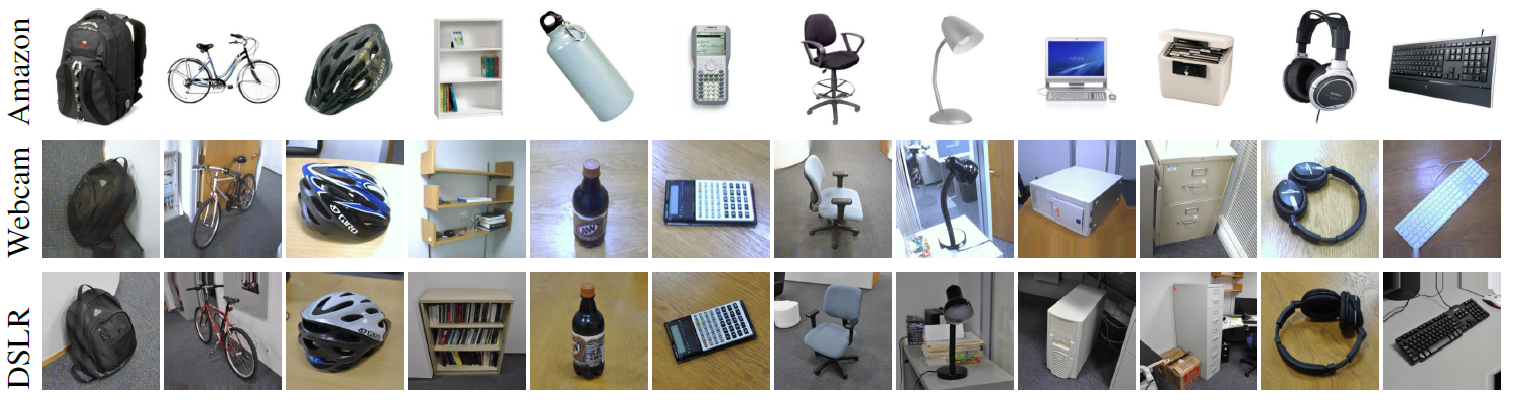
\includegraphics[height=4cm]{images/officeimages.png}
\caption{One kernel at $x_s$ ({\it dotted kernel}) or two kernels at
$x_i$ and $x_j$ ({\it left and right}) }
\label{fig:example}
\end{figure}

\subsubsection{Experimental settings and network design}
On supervised setting, we reused the architecture in people detection. We utilize AlexNet \cite{krizhevsky2012imagenet} as the generic model of both streams. Firstly, we train the source model on source stream with provided training data from Amazon domain. Then iterative algorithm mentioned in Sec \ref{Section:Iterative Algorithm} are utilized for adaptation. The auto-labelling tool takes images on target domain with confidence exceeding 0.9 as training data for next iteration. The difference is besides auto-labelled images on target domain, 3 human labelled images for each class are also included as training data for target model. For each iteration, 100 images are randomly sampled from training data. The unsupervised MMD regularizer added on the element-wise multiply layer transformed from the last full connect layer of target model set the coefficient value $\alpha$ as 10 on Eq \ref{Eq:lmmd}, the same as that in people detection task.

We use the same experimental setting for our unsupervised adaptation, except that at adaptation stage, no human labelled images can be added into the training set.
\subsubsection{Performance evaluation}
In Table x(!), we compare our approach with other six recently published works in both supervised and unsupervised settings. The outstanding performance on both settings confirms the effectiveness of our iterative algorithm and MMD regularizer on the element-wise multiply layer transformed from the last full connect layer.


\begin{table}
\centering
\begin{tabular}{l c c}
  \hline
  % after \\: \hline or \cline{col1-col2} \cline{col3-col4} ...
   & \multicolumn{2}{c}{A $\rightarrow$ W}    \\
   \cline{2-3}
   ~~~~~~~~~~~~~~~~~~~~~~~~~~~~~~~
   ~~~~~~~~~~~~~~~~~~~~~~~~~~~~~~~
    & ~Supervised~ & ~Unsupervised~ \\
  \hline
  GFK(PLS,PCA)\cite{gong2012geodesic} & 46.4 & 15.0 \\
  SA \cite{fernando2013unsupervised} & 45.0 & 15.3 \\
  DA-NBNN \cite{tommasi2013frustratingly} & 52.8 & 23.3 \\
  DLID \cite{chopra2013dlid}& 51.9 & 26.1 \\
  DeCAF${}_{6}$S \cite{donahue2013decaf} & 80.7 & 52.2 \\
  DaNN \cite{ghifary2014domain}& 53.6 & 35.0 \\
  \hline
  Ours & {\bf 84.3} & {\bf 66.3} \\
  Ours & {\bf 85.4} & {\bf 69.3} \\
  \hline
\end{tabular}
\end{table}


\section{Conclusions}
\label{section:Conclusions}

The paper ends with a conclusion.

\begin{figure}
\centering
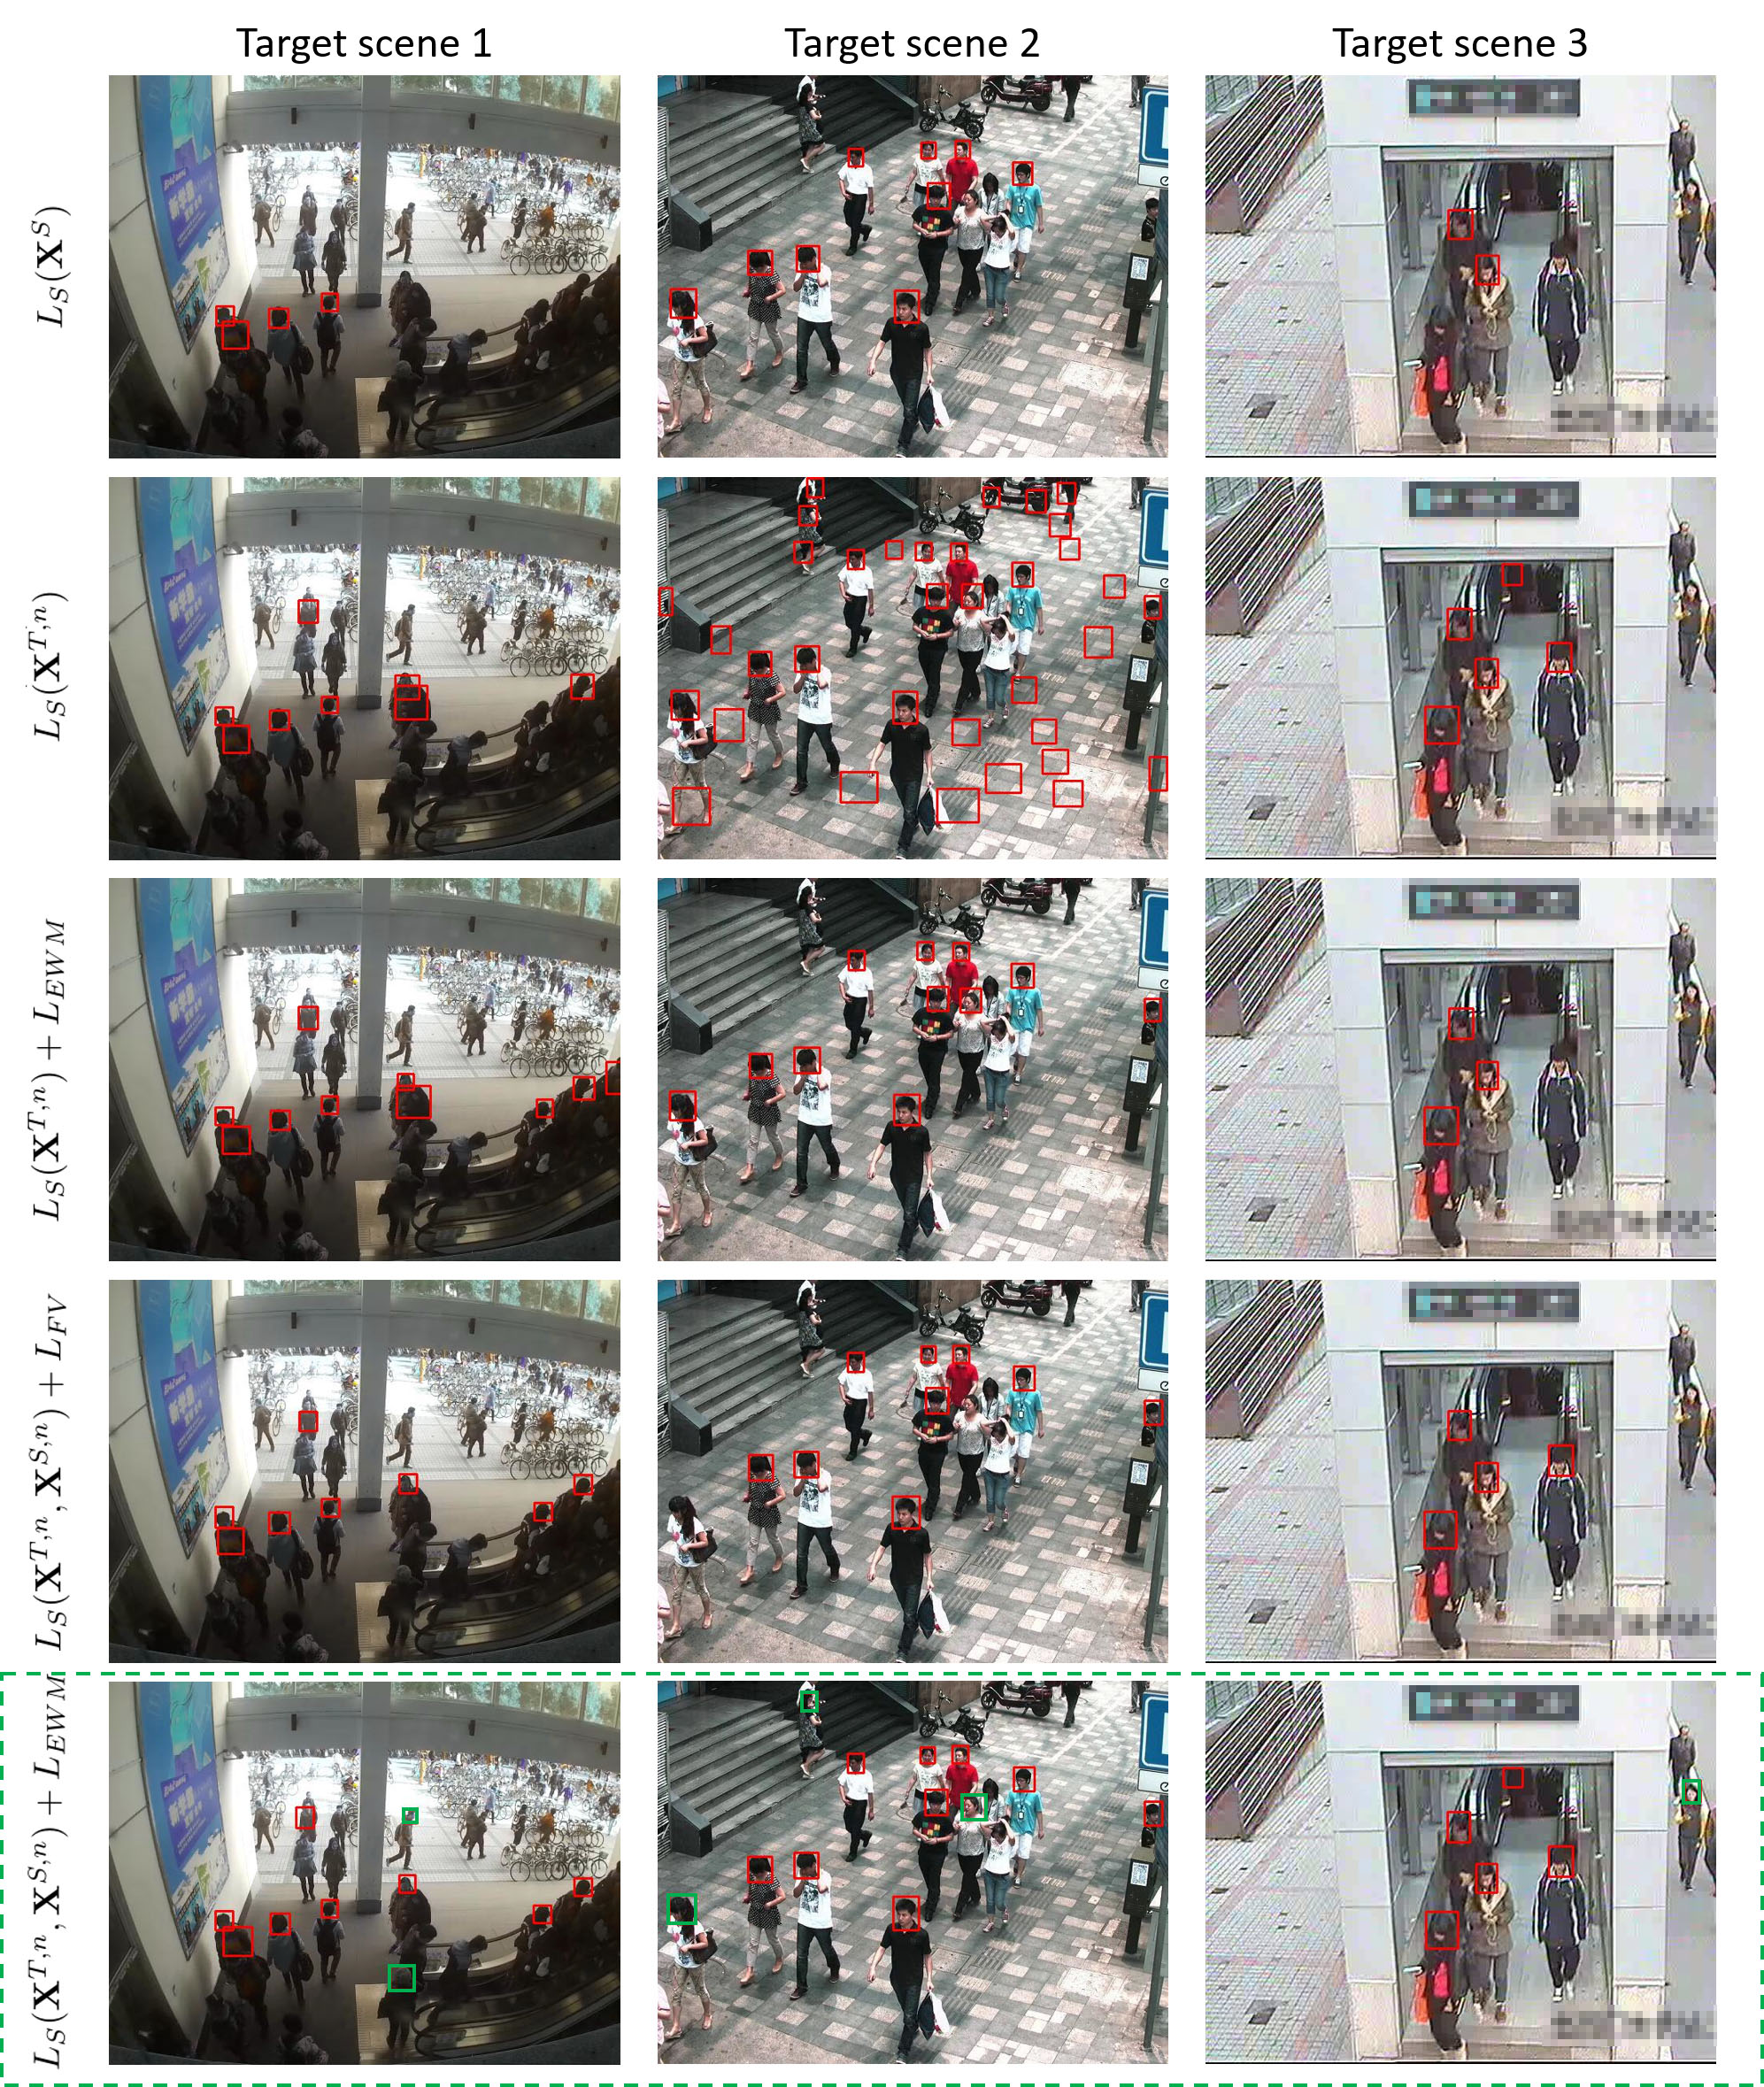
\includegraphics[height=13cm]{images/detectionresult.png}
\caption{One kernel at $x_s$ ({\it dotted kernel}) or two kernels at
$x_i$ and $x_j$ ({\it left and right}) }
\label{fig:example}
\end{figure}

\bibliographystyle{splncs}
\bibliography{egbib}
\end{document}
